\documentclass{article}

\usepackage{amsmath, amsthm, amssymb, amsfonts}
\usepackage{thmtools}
\usepackage{graphicx}
\usepackage{setspace}
\usepackage{geometry}
\usepackage{float}
\usepackage{hyperref}
\usepackage[utf8]{inputenc}
\usepackage[english]{babel}
\usepackage{framed}
\usepackage[dvipsnames]{xcolor}
\usepackage{tcolorbox}
\usepackage{booktabs}
\usepackage{subcaption}

\colorlet{LightGray}{White!90!Periwinkle}
\colorlet{LightOrange}{Orange!15}
\colorlet{LightGreen}{Green!15}

\newcommand{\HRule}[1]{\rule{\linewidth}{#1}}

\setstretch{1.2}
\geometry{
    textheight=9in,
    textwidth=5.5in,
    top=1in,
    headheight=12pt,
    headsep=25pt,
    footskip=30pt
}

% ------------------------------------------------------------------------------

\begin{document}

% ------------------------------------------------------------------------------
% Cover Page and ToC
% ------------------------------------------------------------------------------

\title{ \normalsize \textsc{}
		\\ [2.0cm]
		\HRule{1.5pt} \\
		\LARGE \textbf{\uppercase{E1 294o: Edge and Cloud Systems for Machine Learning Algorithms (Jan`26)}
		\HRule{2.0pt} \\ [0.6cm] \LARGE{Assignment 5} \vspace*{10\baselineskip}}
        
		}
\date{}
\author{\textbf{Author} \\ 
		Ritik Agarwal \\
		MTech DSBA, IISc \\
		19/04/2026}

\maketitle
\newpage

\tableofcontents
\newpage

\section{Strategies}

\begin{itemize}
    \item \textbf{Synchronous:} Both snapshot and persist run on the main thread. Training blocks until the file is written.
\begin{verbatim}
  Train --> Snapshot (blocked) --> Persist (blocked) --> Train
\end{verbatim}

    \item \textbf{Persist Pipeline:} Snapshot runs on the main thread; persist is offloaded to a background thread.
\begin{verbatim}
  Train --> Snapshot --> Train
               \----> Persist (background)
\end{verbatim}

    \item \textbf{Snapshot + Persist Pipeline:} Both snapshot and persist run in a background thread. Training resumes immediately.
\begin{verbatim}
  Train --> Train
       \----> Snapshot --> Persist (background)
\end{verbatim}
\end{itemize}

\subsection{Results and Analysis}

We trained LeNet-5 ($\sim$62K parameters) on MNIST (60K images, batch size 64) with Adam (lr=0.001) for 100 epochs, checkpointing the full model at every epoch.

\begin{table}[h]
\centering
\begin{tabular}{lcc}
\toprule
\textbf{Strategy} & \textbf{Total Time (s)} & \textbf{Avg per Epoch (s)} \\
\midrule
Synchronous              & 6346.92 & 63.47 \\
Persist Pipeline         & 2846.46 & 28.46 \\
Snapshot+Persist Pipeline & 2500.98 & 25.01 \\
\bottomrule
\end{tabular}
\caption{Training time for 100 epochs of LeNet-5 on MNIST.}
\end{table}

\begin{figure}[h]
\centering
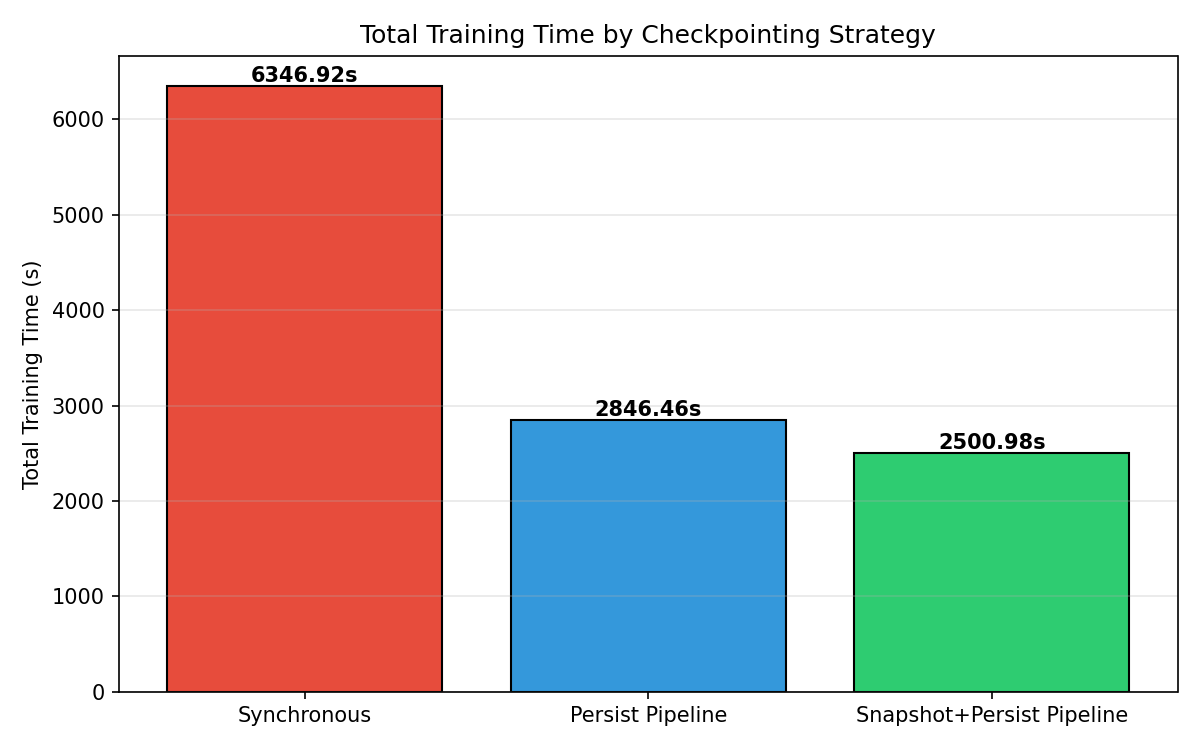
\includegraphics[width=0.7\textwidth]{chart_total_time.png}
\caption{Total training time comparison.}
\end{figure}

\begin{figure}[h]
\centering
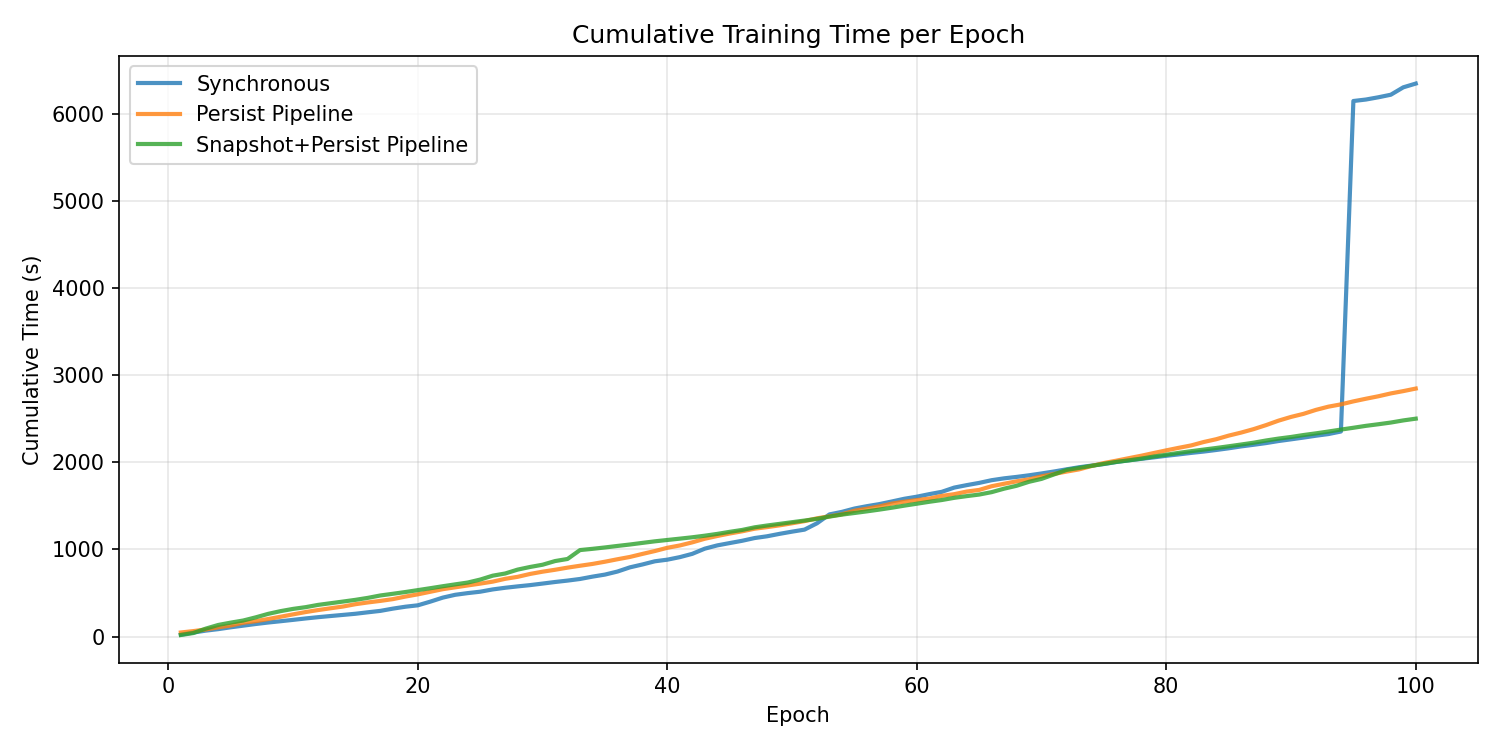
\includegraphics[width=0.8\textwidth]{chart_cumulative_time.png}
\caption{Cumulative training time over 100 epochs.}
\end{figure}

Moving persists to background alone reduces total time by $\sim$55\%, since we don't wait for the high-latency disk writes. However, the small increase with snapshotting in background is expected because the $deepcopy$ operation for a small model like  LeNet-5 is quite cheap. For larger models, the snapshot+persist pipeline would show a bigger advantage.

\end{document}

